\documentclass[paper=a4, fontsize=11pt]{scrartcl} % A4 paper and 11pt font size
\usepackage[utf8]{inputenc}
\usepackage[T1]{fontenc} % Use 8-bit encoding that has 256 glyphs
\usepackage[english]{babel} % English language/hyphenation
\usepackage{amsmath,amsfonts,amsthm} % Math packages

\usepackage{lipsum} % Used for inserting dummy 'Lorem ipsum' text into the template

\usepackage{sectsty} % Allows customizing section commands
\allsectionsfont{\centering \normalfont\scshape} % Make all sections centered, the default font and small caps

\usepackage{fancyhdr} % Custom headers and footers
\pagestyle{fancyplain} % Makes all pages in the document conform to the custom headers and footers
\fancyhead[L]{GROUP 6} % No page header - if you want one, create it in the same way as the footers below
\fancyfoot[L]{} % Empty left footer
\fancyfoot[C]{} % Empty center footer
\fancyfoot[R]{\thepage} % Page numbering for right footer
\renewcommand{\headrulewidth}{0pt} % Remove header underlines
\renewcommand{\footrulewidth}{0pt} % Remove footer underlines
\setlength{\headheight}{13.6pt} % Customize the height of the header

\usepackage{hyperref}
\hypersetup{
    colorlinks,
    citecolor=black,
    filecolor=black,
    linkcolor=black,
    urlcolor=black
}

\numberwithin{equation}{section} % Number equations within sections (i.e. 1.1, 1.2, 2.1, 2.2 instead of 1, 2, 3, 4)
\numberwithin{figure}{section} % Number figures within sections (i.e. 1.1, 1.2, 2.1, 2.2 instead of 1, 2, 3, 4)
\numberwithin{table}{section} % Number tables within sections (i.e. 1.1, 1.2, 2.1, 2.2 instead of 1, 2, 3, 4)

\setlength\parindent{0pt} % Removes all indentation from paragraphs - comment this line for an assignment with lots of text

%----------------------------------------------------------------------------------------
%   TITLE SECTION
%----------------------------------------------------------------------------------------

\newcommand{\horrule}[1]{\rule{\linewidth}{#1}} % Create horizontal rule command with 1 argument of height

\title{ 
\normalfont \normalsize 
\textsc{Norwegian University of Science and Technology} \\ [25pt] % Your university, school and/or department name(s)
\horrule{0.5pt} \\[0.4cm] % Thin top horizontal rule
\huge \textbf{Assignment 1} \\ % The assignment title
TDT4258 \\
\horrule{2pt} \\[0.5cm] % Thick bottom horizontal rule
}

\author{Stian Jensen\\Asbjørn Ottesen Steinskog\\Christoffer Cristea Tønnessen}

\date{\normalsize\today}

\begin{document}

\pagenumbering{roman}

\maketitle

\newpage

%ABSTRACT
\section{Abstract}

This report provides a solution to the first lab exercise in TDT4258 Energy Efficient
Computer Systems. The goal of this exercise was to etc etc program etc energy efficiency etc.. The energy efficiency was an important aspect of this exercise, and by measuring the power consumption in real-time, we were, by the use of interrupts, able to keep it to a minimum.


\newpage

\tableofcontents

\setcounter{secnumdepth}{3}

\newpage

\pagenumbering{arabic}

%INTRODUCTION
\section{Introduction}

In this exercise, a C program that plays sound effects as a response to button pushes on the gamepad was written.

The user is able to play the desired sound effect through pushing different buttons on the gamepad.
Achieving energy efficience through an intelligent use of interrupt handling in the C programming language was one of the main issues in this exercise, and an explanation of our procedure to solve this problem will follow in this report.
Moreover, we will in this report describe how we through sound wave synthesis managed to produce the different sounds.
The explanation of our setup and our code will result in our test results, conclusion, and and evaluation of the assignment.


\newpage

%DESCRIPTION AND METHODOLOGY
\section{Development process and implementation}
\label{chap:development_process}

This chapter details the steps used during the development of the program.
We started by re-implementing most of the code used in the previous exercise, only this time in C.
In addition we set up a timer, which was to be used for interacting with the DAC.

% - setting up interrupts from c
% - embedding assembly

\subsection{Setting up the DAC}

To get sound playing on the board, we had to use the DAC, a Digital-to-Analog Converter.
A timer was needed to be able to continuously write sound samples to the DAC.

\subsection{Timer}

The timer clock frequency is 14MHz, but for the music we only want a freqency of 44100KHz.
Therefore we set the sample period to $ \frac{\SI{14}{\mega\hertz}}{\SI{44100}{\kilo\hertz}} \approx 317 $.

\subsection{Sound synthesis}
The three sound effects we've implemented are all generated in real-time on the board.
We made three different sound effects: a coin blip, a laser, and a level-up sound.
They are all based on a simple waveform, either a square wave or a sawtooth.
Each sound has parameters that are allowed to change for each playback.
Those parameters include frequency, slide, and ADSR parameters.
To leverage the fact that the sound samples are generated on-the-fly, we added a bit of randomization to the ADSR parameters.
This made each playback of a sound effect unique, so each time you press the button for a given sound effect it will sound slightly different.
In addition to varying the ADSR parameters, the frequency was randomized within a given interval for each of the sound effects.
We also added a custom slide to each of them – this allowed the frequency to change gradually during the sound.

\subsubsection{ADSR}

A waveform with constant frequency alone would not provide the sound effects we wanted. We therefore implemented a ADSR envelope \cite{adsr}.
The envelope consists of an attack period, a decay period, a sustain level and a release period, as seen in figure \ref{fig:adsr_envelope}.

\begin{itemize}
    \item The attack periode is the time to use from zero to maximum amplitude.
    \item The decay is the time from max amplitude down to the sustain level.
    \item The sustain level is the amplitude to rest on between the decay and release periods.
    \item The release indicates how much time to spend fading from the sustain level to zero volume.
\end{itemize}

\begin{figure}[ht!]
    \begin{center}
    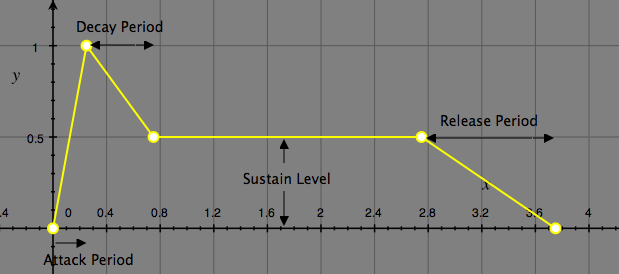
\includegraphics[width=0.8\textwidth]{assets/img/adsr.png}
    \caption{A ADSR envelope}
    \label{fig:adsr_envelope}
    \end{center}
\end{figure}

\subsubsection{Effects}

The parameter intervals for the three implemented sound effects can be seen in Table \ref{tab:sound_effects}.

\begin{table}[ht!]
    \begin{center}
    \begin{tabular}{r|lll}
    Parameter           & Coin       & Laser             & Level-up   \\
    \hline
    Waveform            & Square     & Square / Sawtooth & Sawtooth   \\
    Frequency (initial) & 1500-3000  & 1200-3200         & 100-1100   \\
    Slide               & 0          & -2                & 6          \\
    Attack              & 0          & 0                 & 0-500      \\
    Decay               & 0-3500     & 1000-3000         & 1000-3000  \\
    Sustain level       & 30-80      & 0-50              & 50-100     \\
    Release             & 4000-18000 & 4500-10500        & 2500-16500 \\
    \end{tabular}
    \end{center}
    \caption{Parameter intervals for the implemented sound effects}
    \label{tab:sound_effects}
\end{table}

All sound effect calculations are done with integers, to ensure that the calculations are fast enough to be processed within one timer interval.

\newpage

\subsubsection{Custom random function}

There was no rand() function available, so we made one ourselves:
\\[0.5cm]
\begin{code}

static unsigned int next = 1;

int rand_r(unsigned int *seed) {
    *seed = *seed * 1103515245 + 12345;
    return (*seed % ((unsigned int)RAND_MAX + 1));
}

int rand() {
    return (rand_r(&next));
}


\end{code}

\subsection{Pre-recorded melody}

% Details of exporting from FL Studio, convert to C array

\subsection{Button control}

Buttons are set up to control one sound effect each. The remaining buttons will stop the sound currently playing.


\newpage

%RESULTS AND TEST
\section{Results and Tests}

As mentioned in the description section, we implemented two versions of this program; the first one using polling, where the computer has to check the status of the GPIO repeatedly, and the final version using interrupts, where the program may sleep between its tasks. The version running interrupts is, of course, expected to produce significantly less power consumptive results. Below follows test results for both programs, with a summarizing comparison at the end.

\subsection{Polling}

See figure \ref{fig:polling_io} in the appendices for the power consumption while using polling. The different stages of the program are marked as follows:

Boot sequence: 1.1
Running, no buttons pushed: 1.2
Running, alternating button-pushing: 1.3

Average current while no buttons are pushed: 3.51

\subsection{Interrupt}

Interrupts should result in a more energy-friendly power usage than polling. Below follows results for the two test.

\subsubsection{Without deep sleep}

See figure \ref{fig:interrupt_io} in the appendices for the power consumption while using intterrupts without deep sleep. The different stages of the program are marked as follows:

Boot sequence: 2.1
Running, no buttons pushed: 2.2
Running, alternating button-pushing: 2.3

Average current while no buttons are pushed: 

\subsubsection{With deep sleep}

See figure \ref{fig:interrupt_io_deep_sleep} in the appendices for the power consumption while using interrupts with deep sleep. The different stages of the program are marked as follows:

Boot sequence: 3.1
Running, no buttons pushed: 3.2
Running, alternating button-pushing: 3.3

\subsection{Comparison}

The following table compares the power consumption in the different versions of the implemented programs:




\newpage

%EVALUATION OF ASSIGNMENT
\section{Evaluation of Assignment}

The assignment turned out to be very instructive yet challenging. The compendium introduced the exercise in an informative way, giving useful step-by-step instructions for how to approach the problem, as well as giving eludicative information about the components that we were required to use in this exercise. Using the EFM32 microcontroller was a great way to learn about energy efficiency and how to apply this information in practical situations. The indoor climate at the lab, though, felt pretty bad when the lab got cramped. Sitting hour after hour in a small, cramped room, was exhausting at times. However, the exercise provided a great introduction to energy efficient computer systems. 


\newpage

%CONCLUSION
\section{Conclusion}

The LEDS on the gamepad lights up as intended with both the usage of polling and interrupts when pushed. Multiple ways of energy conservatism was used. And the program managed to solve this task in a very energy efficient way.

The tests were done with energy mode 1 and energy mode 2. There exists an energy mode 3 which conserves 0.2 \si{\mikro\Ampere} less than energy mode 3 \cite{efm32gg-ref-man}. We were not sure if we managed to get into this state, and since the power difference is less than the flucutation when the device is idle, it was very hard to know for sure. The biggest gain in power efficiency is to go from energy mode 1 to energy mode 2, and we did this.

We have, by completing this assignment, gained a greater understanding of not only how to influence the energy efficience, but also of assembly programming, the EFM32 microcontroller, and the GNU toolchain in general. Furthermore, it became clear from the test results that using interrupts and letting the CPU sleep deep when there was no I/O to be processed was a improvement, in regards to power-consumption, over polling.


\newpage

%ACKNOWLEDGEMENTS (THIS IS OPTIONAL)
Acknowledgements goes here.


\newpage

%REFERENCES
\bibliography{bibtexlibs}{}
\bibliographystyle{plain}
\nocite{*}
All resources checked on 2014-02-09



\end{document}
